% Vietnamese translation for OI Public Library
% Source-PDF: IOI中国国家候选队论文/2002/符文杰.pdf
\documentclass[11pt]{article}
\usepackage{oipl-vn}
\usepackage{tikz}
\usetikzlibrary{arrows.meta,decorations.pathreplacing,fit,positioning}
\renewcommand{\figurename}{Hình}

\title{Mạng sắp xếp}
\author{Fu Wenjie}
\date{}

\newcommand{\comp}[3]{%
  \draw (#1,#2) -- (#1,#3);
  \fill (#1,#2) circle (1.6pt);
  \fill (#1,#3) circle (1.6pt);
}
\newcommand{\eightwires}[2]{%
  \foreach \y in {0,-1,-2,-3,-4,-5,-6,-7} {
    \draw (#1,\y) -- (#2,\y);
  }
}

\begin{document}
\maketitle

\origtitle{Sorting networks}
\sourcepath{IOI China candidate team papers / 2002 / Fu Wenjie.pdf}

\section{Mở đầu}

Trước đây ta đã học nhiều thuật toán sắp xếp trên máy tính tuần tự, chẳng hạn
heapsort và quicksort. Loại máy tính đó tại mỗi thời điểm chỉ thực hiện một
thao tác. Bài viết này giới thiệu một mô hình khác: \term{mạng sắp xếp}. Trong
mô hình mạng này, nhiều phép so sánh có thể được thực hiện đồng thời.

Trước hết cần làm rõ một vài khái niệm cơ bản.

\begin{itemize}
  \item \term{Mạng sắp xếp} là một mạng so sánh luôn sắp xếp đúng mọi đầu vào.
  \item \term{Mạng so sánh} chỉ gồm các bộ so sánh và các đường truyền.
  \item Một \term{bộ so sánh} là thiết bị có hai đầu vào $x,y$ và hai đầu ra
  $x',y'$, thực hiện
  \[
    x'=\min(x,y),\qquad y'=\max(x,y).
  \]
  Trong hình vẽ, bộ so sánh thường được biểu diễn bằng một đoạn thẳng đứng nối
  hai đường ngang. Đầu vào nằm bên trái, đầu ra nằm bên phải; giá trị nhỏ hơn
  đi ra ở đường trên, giá trị lớn hơn đi ra ở đường dưới. Vì vậy có thể xem bộ
  so sánh như một phép sắp xếp hai phần tử. Ta giả sử mỗi phép so sánh mất thời
  gian $O(1)$, tức là thời gian từ khi nhận $x,y$ đến khi sinh $x',y'$ là hằng
  số.

  \begin{figure}[ht]
  \centering
  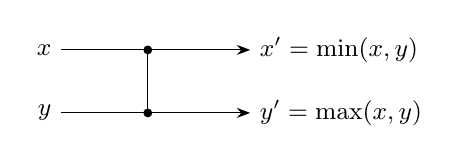
\begin{tikzpicture}[x=1cm,y=1cm,>=Stealth,every node/.style={font=\small}]
    \draw[->] (-0.1,0) -- (2.3,0);
    \draw[->] (-0.1,-0.8) -- (2.3,-0.8);
    \node[left] at (-0.1,0) {$x$};
    \node[left] at (-0.1,-0.8) {$y$};
    \node[right] at (2.3,0) {$x'=\min(x,y)$};
    \node[right] at (2.3,-0.8) {$y'=\max(x,y)$};
    \comp{1.0}{0}{-0.8}
  \end{tikzpicture}
  \caption{Một bộ so sánh hai đầu vào.}
  \end{figure}
  \item \term{Đường truyền} đưa một giá trị từ nơi này sang nơi khác. Nó có thể
  nối đầu ra của một bộ so sánh với đầu vào của một bộ so sánh khác; ngoài ra
  nó có thể là đường vào hoặc đường ra của toàn mạng.
  \item Một \term{mạng so sánh} là tập các bộ so sánh nối với nhau bằng đường
  truyền. Ta vẽ mạng có $n$ đầu vào bằng $n$ đường ngang. Mỗi bộ so sánh nối
  hai đường ngang. Đầu vào của một bộ so sánh hoặc nối với một trong các đường
  vào $a_1,a_2,\ldots,a_n$, hoặc nối với đầu ra của một bộ so sánh khác. Tương
  tự, đầu ra của một bộ so sánh hoặc nối với một trong các đường ra
  $b_1,b_2,\ldots,b_n$, hoặc nối với đầu vào của bộ so sánh khác. Đồ thị nối
  các bộ so sánh không được có chu trình. Một bộ so sánh chỉ sinh đầu ra khi
  cả hai đầu vào của nó đã có giá trị.
\end{itemize}

Khi mọi bộ so sánh đều chạy trong một đơn vị thời gian, \term{thời gian chạy}
của mạng là thời gian từ lúc các đường vào nhận giá trị đến lúc mọi đường ra
nhận được giá trị.

Mạng sắp xếp là mạng so sánh sao cho với mọi dãy đầu vào, dãy đầu ra luôn đơn
điệu tăng:
\[
  b_1\le b_2\le\cdots\le b_n.
\]
Không phải mọi mạng so sánh đều là mạng sắp xếp, nhưng có những mạng nhỏ có
thể kiểm chứng trực tiếp là sắp xếp đúng.

\begin{figure}[ht]
\centering
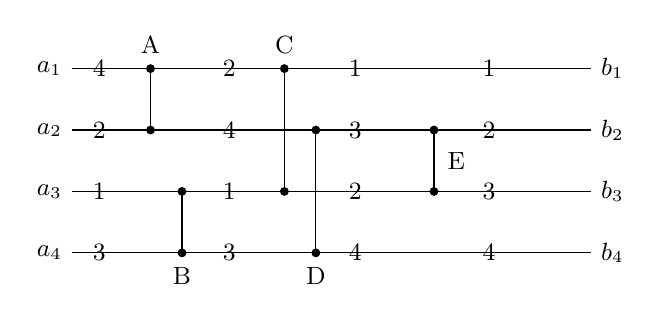
\begin{tikzpicture}[x=1cm,y=0.78cm,every node/.style={font=\small}]
  \foreach \y/\ain/\bout in {0/$a_1$/$b_1$,-1/$a_2$/$b_2$,-2/$a_3$/$b_3$,-3/$a_4$/$b_4$} {
    \draw (0,\y) -- (6.6,\y);
    \node[left] at (0,\y) {\ain};
    \node[right] at (6.6,\y) {\bout};
  }
  \comp{1.0}{0}{-1} \node[above] at (1.0,0.08) {A};
  \comp{1.4}{-2}{-3} \node[below] at (1.4,-3.08) {B};
  \comp{2.7}{0}{-2} \node[above] at (2.7,0.08) {C};
  \comp{3.1}{-1}{-3} \node[below] at (3.1,-3.08) {D};
  \comp{4.6}{-1}{-2} \node[right] at (4.65,-1.5) {E};
  \foreach \x/\vals in {0.35/{4,2,1,3},2.0/{2,4,1,3},3.6/{1,3,2,4},5.3/{1,2,3,4}} {
    \foreach \v [count=\i from 0] in \vals {
      \node at (\x,-\i) {\v};
    }
  }
\end{tikzpicture}
\caption{Một mạng so sánh bốn đầu vào. Với dữ liệu minh họa này, giá trị đầu
ra đã được sắp thành thứ tự tăng.}
\end{figure}

Mạng so sánh giống thủ tục ở chỗ nó chỉ rõ các phép so sánh cần thực hiện.
Điểm khác biệt là kích thước thật sự của mạng phụ thuộc vào số đầu vào và đầu
ra. Vì thế ta thực chất đang mô tả một \term{họ} mạng so sánh. Mục tiêu là tìm
một họ mạng sắp xếp hiệu quả, ký hiệu là \texttt{SORTER}; mạng trong họ này có
$n$ đầu vào và $n$ đầu ra được ký hiệu là \texttt{SORTER[$n$]}.

\section{Nguyên lý 0--1}

Trước khi xây dựng \texttt{SORTER}, ta cần biết cách kiểm tra một mạng so sánh
có phải mạng sắp xếp hay không. Theo định nghĩa, một mạng có $n$ đầu vào là
mạng sắp xếp nếu mọi dãy đầu vào đều cho dãy đầu ra tăng. Nếu kiểm tra trực
tiếp, ta phải xét $n!$ hoán vị đầu vào, khối lượng rất lớn.

Kết quả quan trọng giúp đơn giản hóa việc kiểm tra là \term{nguyên lý 0--1}:
nếu một mạng so sánh sắp xếp đúng mọi dãy đầu vào chỉ gồm $0$ và $1$, thì nó
sắp xếp đúng mọi dãy giá trị tùy ý. Ta chứng minh nguyên lý này qua một bổ đề.

\paragraph{Bổ đề 1.}
Giả sử mạng so sánh biến dãy đầu vào
\[
  a=\langle a_1,a_2,\ldots,a_n\rangle
\]
thành dãy đầu ra
\[
  b=\langle b_1,b_2,\ldots,b_n\rangle.
\]
Với mọi hàm đơn điệu không giảm $f$, mạng đó biến
\[
  f(a)=\langle f(a_1),f(a_2),\ldots,f(a_n)\rangle
\]
thành
\[
  f(b)=\langle f(b_1),f(b_2),\ldots,f(b_n)\rangle.
\]

\paragraph{Chứng minh.}
Ta quy nạp theo số bộ so sánh $m$ trong mạng.

Với $m=1$, giả sử bộ so sánh nối $a_i$ và $a_j$. Khi đầu vào là $a_i,a_j$, đầu
ra trên là $\min(a_i,a_j)$ và đầu ra dưới là $\max(a_i,a_j)$. Nếu thay đầu vào
bằng $f(a_i),f(a_j)$, vì $f$ đơn điệu không giảm, ta có
\[
  \min(f(a_i),f(a_j))=f(\min(a_i,a_j)),
\]
\[
  \max(f(a_i),f(a_j))=f(\max(a_i,a_j)).
\]
Do đó bổ đề đúng khi chỉ có một bộ so sánh.

Giả sử bổ đề đúng với mọi mạng có ít hơn $k$ bộ so sánh, xét mạng có $k$ bộ so
sánh. Tách mạng thành hai mạng nối tiếp: $S_1$ gồm $k-1$ bộ so sánh đầu tiên,
và $S_2$ là bộ so sánh cuối cùng. Nếu $S_1$ biến $a$ thành
$c=\langle c_1,c_2,\ldots,c_n\rangle$, rồi $S_2$ biến $c$ thành $b$, thì theo
giả thiết quy nạp, đầu vào $f(a)$ đi qua $S_1$ sẽ thành $f(c)$, và $f(c)$ đi
qua $S_2$ sẽ thành $f(b)$. Vậy bổ đề cũng đúng với $m=k$, suy ra đúng với mọi
mạng hữu hạn.

\paragraph{Nguyên lý 0--1.}
Nếu một mạng so sánh có $n$ đầu vào sắp xếp đúng mọi dãy trong $\{0,1\}^n$, thì
nó sắp xếp đúng mọi dãy giá trị tùy ý.

\paragraph{Chứng minh.}
Chứng minh phản chứng. Giả sử mạng sắp xếp đúng mọi dãy 0--1 nhưng không sắp
xếp đúng một dãy giá trị tùy ý. Khi đó tồn tại đầu vào mà ở đầu ra có hai phần
tử $a_i<a_j$ nhưng $a_j$ đứng trước $a_i$. Định nghĩa hàm đơn điệu không giảm
\[
  f(x)=
  \begin{cases}
    0, & x\le a_i,\\
    1, & x>a_i.
  \end{cases}
\]
Theo bổ đề 1, khi đưa dãy $f(a)$ vào mạng, thứ tự tương ứng ở đầu ra vẫn có
$f(a_j)$ đứng trước $f(a_i)$. Nhưng $f(a_j)=1$ và $f(a_i)=0$, nên đầu ra của
dãy 0--1 này không được sắp xếp. Điều đó mâu thuẫn với giả thiết. Nguyên lý
được chứng minh.

Khi xây dựng mạng sắp xếp và các mạng so sánh khác, nguyên lý 0--1 cho phép ta
chỉ tập trung vào các dãy gồm $0$ và $1$. Một khi chứng minh được mạng sắp xếp
đúng mọi dãy 0--1, ta lập tức suy ra nó sắp xếp đúng mọi dãy giá trị.

\section{Từ sắp xếp đến trộn}

Nguyên lý 0--1 giúp việc kiểm tra dễ hơn, nhưng ta vẫn cần xây dựng một họ
mạng sắp xếp. Với một mạng \texttt{SORTER[$n$]}, nếu cố xây dựng trực tiếp từ
đầu thì khá khó. Ta dùng tư tưởng chia đôi: chia $n$ phần tử thành hai nửa, lần
lượt sắp xếp bằng hai mạng \texttt{SORTER[$n/2$]}, rồi dùng một mạng
\texttt{MERGER[$n$]} để trộn hai dãy tăng thành một dãy tăng. Bài toán chính
vì vậy chuyển thành xây dựng họ mạng trộn \texttt{MERGER[$n$]}.

Nếu ghép một dãy tăng với một dãy giảm, ta thu được một \term{dãy song điệu}
(\emph{bitonic sequence}). Một dãy song điệu là dãy trước tăng rồi sau giảm,
hoặc trước giảm rồi sau tăng. Ví dụ
\[
  \langle 1,4,6,8,3,2\rangle,\qquad
  \langle 9,8,3,2,4,6\rangle
\]
đều là song điệu. Với dãy chỉ gồm $0$ và $1$, cấu trúc song điệu đơn giản hơn:
nó có dạng $0^i1^j0^k$ hoặc $1^i0^j1^k$, với $i,j,k\ge 0$.

Các tính chất của dãy song điệu giúp ta xây dựng mạng sắp xếp song điệu.

\section{Bộ nửa làm sạch}

Mạng sắp xếp song điệu gồm $\log_2 n$ giai đoạn; mỗi giai đoạn là một
\term{bộ nửa làm sạch} (\emph{half-cleaner}). Với $n$ chẵn, bộ nửa làm sạch là
mạng có độ sâu $1$ gồm các bộ so sánh giữa đường vào $i$ và đường vào
$i+n/2$, với $i=1,2,\ldots,n/2$.

\begin{figure}[ht]
\centering
\begin{tikzpicture}[x=1cm,y=0.56cm,every node/.style={font=\small}]
  \eightwires{0}{5.8}
  \foreach \y/\vin/\vout in {
    0/0/0,-1/0/0,-2/1/0,-3/1/0,
    -4/1/1,-5/0/0,-6/0/1,-7/0/1} {
    \node[left] at (0,\y) {\vin};
    \node[right] at (5.8,\y) {\vout};
  }
  \foreach \i/\j in {0/-4,-1/-5,-2/-6,-3/-7} {\comp{2.9}{\i}{\j}}
  \node[left,align=center] at (-0.7,-3.5) {dãy\\song điệu};
  \node[right,align=center] at (6.4,-1.5) {dãy song điệu\\sạch};
  \node[right,align=center] at (6.4,-5.5) {dãy song điệu};
\end{tikzpicture}
\caption{Bộ nửa làm sạch có tám đầu vào: so sánh từng cặp tương ứng giữa hai
nửa của dãy.}
\end{figure}

Khi đầu vào là một dãy song điệu 0--1, đầu ra của bộ nửa làm sạch thỏa ba tính
chất:
\begin{itemize}
  \item các giá trị nhỏ hơn nằm ở nửa trên, các giá trị lớn hơn nằm ở nửa
  dưới;
  \item hai nửa đầu ra vẫn là các dãy song điệu;
  \item ít nhất một trong hai nửa là \term{sạch}, tức toàn $0$ hoặc toàn $1$.
\end{itemize}

\paragraph{Định lý 1.}
Nếu đầu vào của một bộ nửa làm sạch là một dãy song điệu gồm $0$ và $1$, thì
nửa trên và nửa dưới của đầu ra đều song điệu; mọi phần tử ở nửa trên không
lớn hơn mọi phần tử ở nửa dưới; và ít nhất một trong hai nửa là sạch.

\paragraph{Chứng minh.}
Không mất tính tổng quát, xét đầu vào dạng
\[
  00\cdots 011\cdots 100\cdots 0.
\]
Dạng còn lại $11\cdots 100\cdots 011\cdots 1$ là đối xứng. Tùy vị trí trung
điểm $n/2$ nằm trong đoạn liên tiếp các số $0$ hay đoạn liên tiếp các số $1$,
ta có ba trường hợp lớn; trường hợp trung điểm nằm trong đoạn các số $1$ lại
tách thành hai trường hợp nhỏ. Trong từng trường hợp, mỗi phép so sánh ghép
một phần tử ở nửa trên với một phần tử tương ứng ở nửa dưới. Phần tử nhỏ hơn
được đưa lên trên và phần tử lớn hơn được đưa xuống dưới, nên nửa trên không
lớn hơn nửa dưới. Do dãy ban đầu chỉ có nhiều nhất hai lần đổi giá trị giữa
$0$ và $1$, sau các phép so sánh song song, mỗi nửa vẫn có cấu trúc song điệu.
Quan sát các vị trí của đoạn giữa cho thấy một trong hai nửa không còn chứa cả
hai giá trị, tức là sạch. Định lý được chứng minh.

\begin{figure}[ht]
\centering
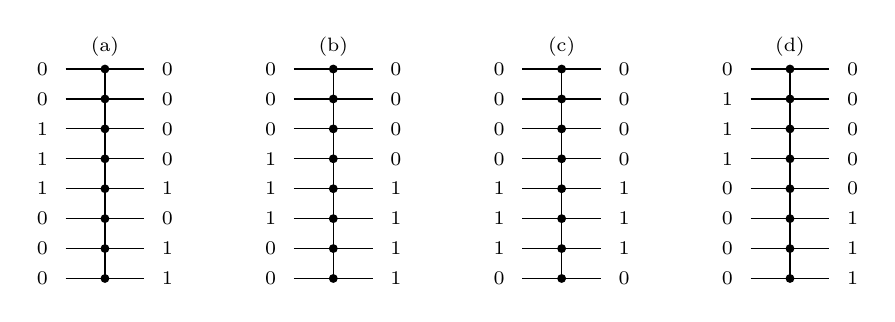
\begin{tikzpicture}[x=1cm,y=0.38cm,every node/.style={font=\scriptsize}]
  \foreach \x/\name in {0/(a),2.9/(b),5.8/(c),8.7/(d)} {
    \node at (\x+1.05,0.75) {\name};
    \foreach \i in {0,...,7} {
      \draw (\x+0.55,-\i) -- (\x+1.55,-\i);
    }
    \foreach \i/\j in {0/-4,-1/-5,-2/-6,-3/-7} {\comp{\x+1.05}{\i}{\j}}
  }
  \foreach \i/\v in {0/0,1/0,2/1,3/1,4/1,5/0,6/0,7/0}
    \node[left] at (0.45,-\i) {\v};
  \foreach \i/\v in {0/0,1/0,2/0,3/0,4/1,5/0,6/1,7/1}
    \node[right] at (1.65,-\i) {\v};
  \foreach \i/\v in {0/0,1/0,2/0,3/1,4/1,5/1,6/0,7/0}
    \node[left] at (3.35,-\i) {\v};
  \foreach \i/\v in {0/0,1/0,2/0,3/0,4/1,5/1,6/1,7/1}
    \node[right] at (4.55,-\i) {\v};
  \foreach \i/\v in {0/0,1/0,2/0,3/0,4/1,5/1,6/1,7/0}
    \node[left] at (6.25,-\i) {\v};
  \foreach \i/\v in {0/0,1/0,2/0,3/0,4/1,5/1,6/1,7/0}
    \node[right] at (7.45,-\i) {\v};
  \foreach \i/\v in {0/0,1/1,2/1,3/1,4/0,5/0,6/0,7/0}
    \node[left] at (9.15,-\i) {\v};
  \foreach \i/\v in {0/0,1/0,2/0,3/0,4/0,5/1,6/1,7/1}
    \node[right] at (10.35,-\i) {\v};
\end{tikzpicture}
\caption{Bốn trường hợp điển hình trong chứng minh của bộ nửa làm sạch. Vị
trí của điểm giữa trong dãy $0^i1^j0^k$ quyết định nửa nào trở thành sạch,
nhưng cấu trúc song điệu của cả hai nửa vẫn được giữ.}
\end{figure}

\section{Mạng sắp xếp song điệu}

Bằng cách nối đệ quy các bộ nửa làm sạch, ta xây dựng được mạng sắp xếp song
điệu. Giai đoạn đầu của \texttt{BITONIC-SORTER[$n$]} là bộ nửa làm sạch kích
thước $n$. Theo định lý 1, nó tạo ra hai dãy song điệu kích thước $n/2$ và mọi
phần tử ở nửa trên không lớn hơn mọi phần tử ở nửa dưới. Vì vậy chỉ cần dùng
hai mạng \texttt{BITONIC-SORTER[$n/2$]} để sắp xếp đệ quy hai nửa là thu được
toàn bộ dãy tăng.

\begin{figure}[ht]
\centering
\begin{tikzpicture}[x=1cm,y=0.7cm,>=Stealth,every node/.style={font=\small}]
  \node[draw,minimum width=1.8cm,minimum height=3.9cm,align=center] (hc)
    at (0,-1.75) {bộ nửa\\làm sạch\\$[n]$};
  \node[draw,minimum width=2.5cm,minimum height=1.5cm,align=center] (top)
    at (3.3,-0.7) {\texttt{BITONIC}\\\texttt{-SORTER[$n/2$]}};
  \node[draw,minimum width=2.5cm,minimum height=1.5cm,align=center] (bot)
    at (3.3,-2.8) {\texttt{BITONIC}\\\texttt{-SORTER[$n/2$]}};
  \draw[->] (-2.0,-1.75) -- (hc.west);
  \draw[->] (hc.east |- top.west) -- (top.west);
  \draw[->] (hc.east |- bot.west) -- (bot.west);
  \draw[->] (top.east) -- (5.5,-0.7);
  \draw[->] (bot.east) -- (5.5,-2.8);
  \node[left,align=center] at (-2.0,-1.75) {dãy\\song điệu};
  \node[right,align=center] at (5.5,-1.75) {dãy\\tăng};
\end{tikzpicture}
\caption{Cấu trúc đệ quy của mạng sắp xếp song điệu.}
\end{figure}

Độ sâu của mạng sắp xếp song điệu là $\log_2 n$, nếu tính riêng bài toán sắp
xếp một dãy song điệu đã cho.

\section{Mạng trộn}

Ta chỉ cần sửa bộ nửa làm sạch đầu tiên của mạng sắp xếp song điệu để thu được
mạng trộn \texttt{MERGER[$n$]}. Đầu vào của \texttt{MERGER[$n$]} gồm hai dãy
tăng, mỗi dãy dài $n/2$. Nếu đảo ngược nửa dưới, hai nửa ghép lại thành một
dãy song điệu. Thêm bộ nửa làm sạch rồi đảo ngược trở lại, bộ nửa làm sạch
tương ứng sẽ so sánh
\[
  a_i\quad\text{với}\quad a_{n-i+1}
  \qquad (i=1,2,\ldots,n/2).
\]
Sau bước này, hai nửa đầu ra vẫn là các dãy song điệu có tính chất nửa trên
không lớn hơn nửa dưới. Vì một dãy song điệu sau khi đảo ngược vẫn là song
điệu, ta có thể tiếp tục dùng hai mạng sắp xếp song điệu kích thước $n/2$ để
hoàn tất việc trộn.

Tóm lại, \texttt{MERGER[$n$]} được xây dựng từ một tầng so sánh giữa các cặp
đối xứng $a_i,a_{n-i+1}$, rồi hai mạng sắp xếp song điệu kích thước $n/2$.

\begin{figure}[ht]
\centering
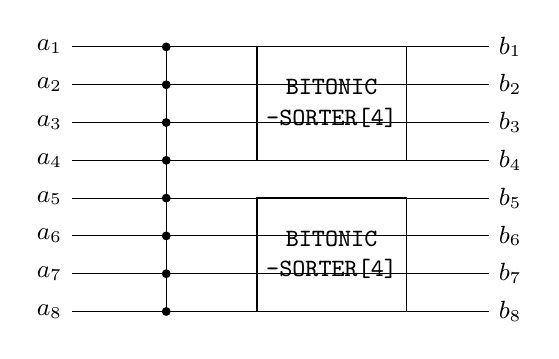
\begin{tikzpicture}[x=1cm,y=0.48cm,every node/.style={font=\small}]
  \eightwires{0}{5.3}
  \foreach \y/\ain/\bout in {
    0/$a_1$/$b_1$,-1/$a_2$/$b_2$,-2/$a_3$/$b_3$,-3/$a_4$/$b_4$,
    -4/$a_5$/$b_5$,-5/$a_6$/$b_6$,-6/$a_7$/$b_7$,-7/$a_8$/$b_8$} {
    \node[left] at (0,\y) {\ain};
    \node[right] at (5.3,\y) {\bout};
  }
  \foreach \i/\j in {0/-7,-1/-6,-2/-5,-3/-4} {\comp{1.2}{\i}{\j}}
  \node[draw,minimum width=1.8cm,minimum height=1.45cm,align=center]
    at (3.3,-1.5) {\texttt{BITONIC}\\\texttt{-SORTER[4]}};
  \node[draw,minimum width=1.8cm,minimum height=1.45cm,align=center]
    at (3.3,-5.5) {\texttt{BITONIC}\\\texttt{-SORTER[4]}};
\end{tikzpicture}
\caption{Cấu trúc của mạng trộn \texttt{MERGER[8]}: tầng đầu so sánh các cặp
đối xứng, sau đó sắp xếp song điệu hai nửa.}
\end{figure}

\section{Xây dựng \texttt{SORTER}}

Họ mạng sắp xếp cuối cùng được định nghĩa đệ quy:
\[
  \texttt{SORTER}[n]
  =
  \texttt{MERGER}[n]\circ
  \bigl(\texttt{SORTER}[n/2]\ \|\ \texttt{SORTER}[n/2]\bigr),
\]
trong đó hai mạng \texttt{SORTER[$n/2$]} chạy song song trên hai nửa đầu vào,
sau đó kết quả được đưa vào \texttt{MERGER[$n$]}. Biên đệ quy là $n=2$.

\begin{figure}[ht]
\centering
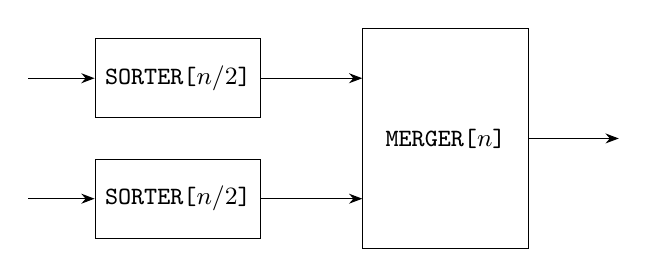
\begin{tikzpicture}[x=1cm,y=0.85cm,>=Stealth,every node/.style={font=\small}]
  \node[draw,minimum width=2.1cm,minimum height=1.0cm,align=center] (top)
    at (0,0) {\texttt{SORTER[$n/2$]}};
  \node[draw,minimum width=2.1cm,minimum height=1.0cm,align=center] (bot)
    at (0,-1.8) {\texttt{SORTER[$n/2$]}};
  \node[draw,minimum width=2.1cm,minimum height=2.8cm,align=center] (merge)
    at (3.4,-0.9) {\texttt{MERGER[$n$]}};
  \draw[->] (-1.9,0) -- (top.west);
  \draw[->] (-1.9,-1.8) -- (bot.west);
  \draw[->] (top.east) -- (merge.west |- top.east);
  \draw[->] (bot.east) -- (merge.west |- bot.east);
  \draw[->] (merge.east) -- (5.6,-0.9);
\end{tikzpicture}
\caption{Cấu trúc đệ quy của \texttt{SORTER[$n$]}.}
\end{figure}

Với $n=8$, mạng được tạo bằng cách ghép các \texttt{MERGER[2]},
\texttt{MERGER[4]} và \texttt{MERGER[8]} theo đúng cây đệ quy trên. Bài gốc
minh họa chi tiết quá trình giá trị 0--1 đi qua các tầng mạng; Hình~\ref{fig:sorter-eight}
giữ lại cấu trúc này và cho thấy sau mỗi giai đoạn, các khối con đã được trộn
thành những dãy tăng dài hơn.

\begin{figure}[ht]
\centering
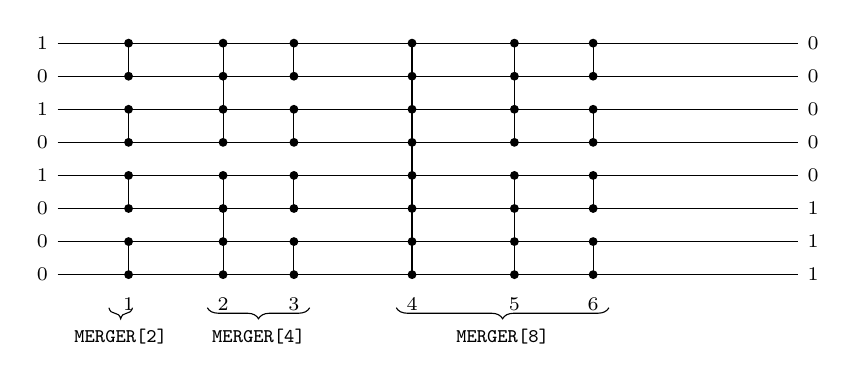
\begin{tikzpicture}[x=1cm,y=0.42cm,every node/.style={font=\scriptsize}]
  \eightwires{0}{9.4}
  \foreach \y/\lab in {0/$1$,-1/$0$,-2/$1$,-3/$0$,-4/$1$,-5/$0$,-6/$0$,-7/$0$}
    \node[left] at (0,\y) {\lab};
  \foreach \y/\lab in {0/$0$,-1/$0$,-2/$0$,-3/$0$,-4/$0$,-5/$1$,-6/$1$,-7/$1$}
    \node[right] at (9.4,\y) {\lab};
  \foreach \a/\b in {0/-1,-2/-3,-4/-5,-6/-7} {\comp{0.9}{\a}{\b}}
  \foreach \a/\b in {0/-3,-1/-2,-4/-7,-5/-6} {\comp{2.1}{\a}{\b}}
  \foreach \a/\b in {0/-1,-2/-3,-4/-5,-6/-7} {\comp{3.0}{\a}{\b}}
  \foreach \a/\b in {0/-7,-1/-6,-2/-5,-3/-4} {\comp{4.5}{\a}{\b}}
  \foreach \a/\b in {0/-3,-1/-2,-4/-7,-5/-6} {\comp{5.8}{\a}{\b}}
  \foreach \a/\b in {0/-1,-2/-3,-4/-5,-6/-7} {\comp{6.8}{\a}{\b}}
  \node[below] at (0.9,-7.4) {1};
  \node[below] at (2.1,-7.4) {2};
  \node[below] at (3.0,-7.4) {3};
  \node[below] at (4.5,-7.4) {4};
  \node[below] at (5.8,-7.4) {5};
  \node[below] at (6.8,-7.4) {6};
  \draw[decorate,decoration={brace,mirror,amplitude=4pt}] (0.65,-8.0) -- (0.95,-8.0)
    node[midway,below=4pt] {\texttt{MERGER[2]}};
  \draw[decorate,decoration={brace,mirror,amplitude=4pt}] (1.9,-8.0) -- (3.2,-8.0)
    node[midway,below=4pt] {\texttt{MERGER[4]}};
  \draw[decorate,decoration={brace,mirror,amplitude=4pt}] (4.3,-8.0) -- (7.0,-8.0)
    node[midway,below=4pt] {\texttt{MERGER[8]}};
\end{tikzpicture}
\caption{Một mạng sắp xếp tám đầu vào được ghép từ các mạng trộn kích thước
$2$, $4$ và $8$.}
\label{fig:sorter-eight}
\end{figure}

Trong \texttt{SORTER[$n$]}, dữ liệu đi qua $\log_2 n$ giai đoạn. Giai đoạn thứ
$K$, với $1\le K\le \log_2 n$, gồm $n/2^K$ mạng \texttt{MERGER[$2^K$]} chạy
song song; mỗi mạng trộn hai dãy tăng độ dài $2^{K-1}$ thành một dãy tăng độ
dài $2^K$. Độ sâu của giai đoạn này là $K$. Vì vậy tổng độ sâu là
\[
  \sum_{K=1}^{\log_2 n}K=O(\log^2 n).
\]
Do đó trong mô hình song song của mạng so sánh, ta có thể sắp xếp $n$ số trong
thời gian $O(\log^2 n)$.

\section{Tổng kết}

Trong quá trình giải bài toán mạng sắp xếp, ta đã nhiều lần thu hẹp và chuyển
hóa vấn đề. Trước hết, nguyên lý 0--1 giảm mạnh phạm vi đầu vào cần xét. Sau
đó, dùng tư tưởng chia đôi để biến sắp xếp một dãy thành sắp xếp hai nửa rồi
trộn chúng. Bài toán tiếp tục chuyển thành xây dựng mạng trộn. Tiếp theo, bộ
nửa làm sạch biến một dãy song điệu thành hai dãy song điệu nhỏ hơn, đồng
thời bảo đảm mọi giá trị ở nửa trên không lớn hơn mọi giá trị ở nửa dưới. Đây
là lần thứ hai tư tưởng chia đôi được dùng. Nhờ gọi đệ quy bộ nửa làm sạch, ta
có mạng sắp xếp song điệu; nhờ đó mạng trộn được giải quyết. Cuối cùng, bằng
cách gọi đệ quy mạng trộn, ta xây dựng được họ mạng sắp xếp.

Những kỹ thuật như thu hẹp phạm vi, chia đôi, và gọi đệ quy kết quả đã có đều
đóng vai trò quan trọng. Dùng chúng khéo léo thường giúp việc giải bài toán
trở nên hiệu quả hơn rất nhiều.

\end{document}
